\documentclass{article}
\usepackage[utf8]{inputenc}
\usepackage{amsmath}
\usepackage{listings}
\usepackage{color}
\usepackage{float}
\usepackage{hyperref}
\usepackage{graphicx}
\usepackage{caption}
\usepackage{subcaption}
\usepackage{adjustbox}
\graphicspath{{Images/}}

\definecolor{codebg}{gray}{0.95}

\lstset{ 
	language=Matlab,                		% choose the language of the code
%	basicstyle=10pt,       				% the size of the fonts that are used for the code
	numbers=left,                  			% where to put the line-numbers
	numberstyle=\footnotesize,      		% the size of the fonts that are used for the line-numbers
	stepnumber=1,                   			% the step between two line-numbers. If it's 1 each line will be numbered
	numbersep=5pt,                  		% how far the line-numbers are from the code
	backgroundcolor=\color{codebg},  	% choose the background color. You must add \usepackage{color}
	showspaces=false,               		% show spaces adding particular underscores
	showstringspaces=false,         		% underline spaces within strings
	showtabs=false,                 			% show tabs within strings adding particular underscores
%	frame=single,	                			% adds a frame around the code
%	tabsize=2,                				% sets default tabsize to 2 spaces
%	captionpos=b,                   			% sets the caption-position to bottom
	breaklines=true,                			% sets automatic line breaking
	breakatwhitespace=false,        		% sets if automatic breaks should only happen at whitespace
	escapeinside={\%*}{*)}          		% if you want to add a comment within your code
}

\title{\textbf{CSE 848 Home Assignment 1}}
\author{\textbf{\textit{Submitted by:}} Ritam Guha (MSU ID: guharita)}
\date{\textbf{\textit{Date:}} January 26, 2021}

\begin{document}

\maketitle

1. We are interested in finding the minimum solution of the following five-variable (n = 5) Rastrigin function starting from 100 random initial points in $x_{i} \epsilon[-5.12, 5.12]$:

\begin{equation*}
    f(x) = 10n + \sum_{x=1}^{n} {x_{i}^2 - 10\cos(\alpha \pi x_i) }
\end{equation*}

Use $\alpha$ = 0.25, 1.0, and 2.0. Apply \textit{fminsearch()} to solve each instance with maximum function evaluations of 5,000 and maximum iterations of 2,000 for each run. For each $\alpha$, report the best solution of 100 runs. Can you explain the results obtained?\\

\textbf{Solution:}
The given Rastrigin function constructs a 5-dimensional ($n=5$) multivariable, unconstrained minimization problem. So, Nelder-Mead's simplex search algorithm can be used to solve this problem. The algorithm has an implementation under the name \textit{fminsearch()} in MATLAB. As suggested in the question, the maximum number of function evaluations and maximum number of allowable iterations have been set to 5000 and 2000 respectively. following code snippet has been used to solve the given optimization problem.\\

\lstinputlisting[language=Matlab]{Codes/q1.m}

After running \textit{fminsearch()} with 100 different initializations for different values of $\alpha$, the best solutions have been tabulated in \autoref{tab:RastriginSolution}. In order to demonstrate the convergence prowess of \textit{fminsearch()}, the reduction in the functional value over the iterations for a single run with $\alpha$=0.25, 1.0 and 2.0 are displayed in \autoref{fig:UncOptimizationPlot}.

\begin{table}[H]
    \centering
    \begin{tabular}{|c|c|c|}
    \hline
        \textbf{$\alpha$} & \textbf{Min f(x)} & \textbf{x} \\ \hline
        0.25 & 4.05E-09 & -1.6056e-05, 2.0453e-05, -1.1009e-06, 1.2019e-05, -1.3062e-05 \\ \hline
        1.0 & 7.8409 & -2.9483e-05, 2.8664e-05, 1.9602, 8.6819e-07, -1.9602 \\ \hline
        2.0 & 13.9294 & 3.5673e-05, -4.1348e-05, -0.99493, 2.9849, -1.9899 \\ \hline
    \end{tabular}
    \caption{The min f(x) and corresponding x obtained after 100 runs of \textit{fminsearch()} with different values of $\alpha$}
    \label{tab:RastriginSolution}
\end{table}

\begin{figure}[H]
    \centering
     \resizebox{0.75\textwidth}{!}{
    \begin{tabular}{c}
        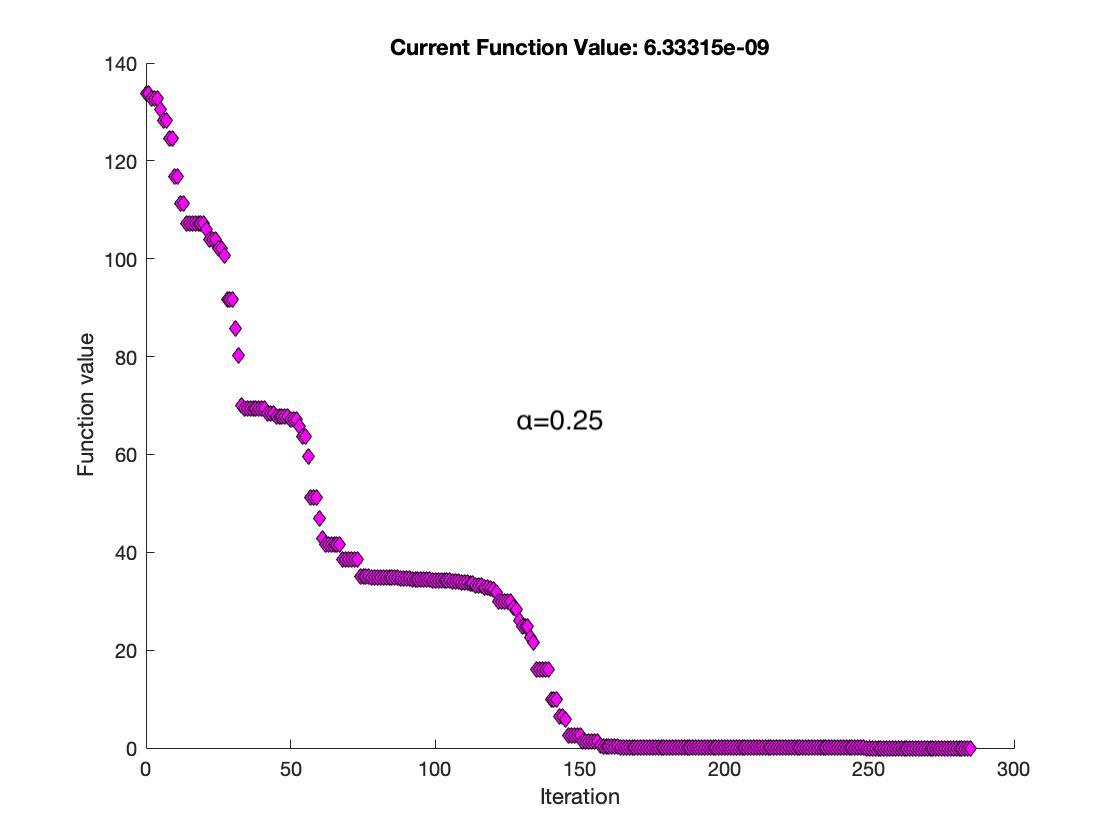
\includegraphics{CSE 848/HA1/Images/q1-Optimization Plot alpha_0.25.jpg}\\ 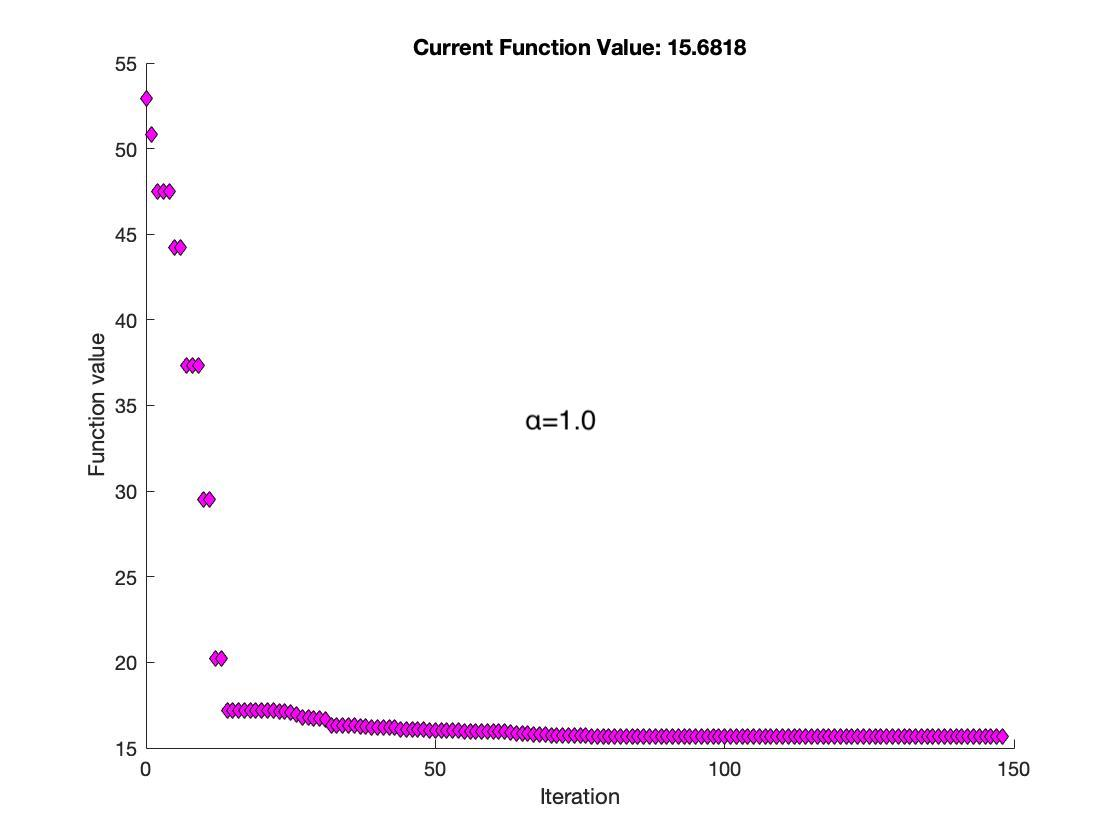
\includegraphics{CSE 848/HA1/Images/q1-Optimization Plot alpha_1.jpg}\\
        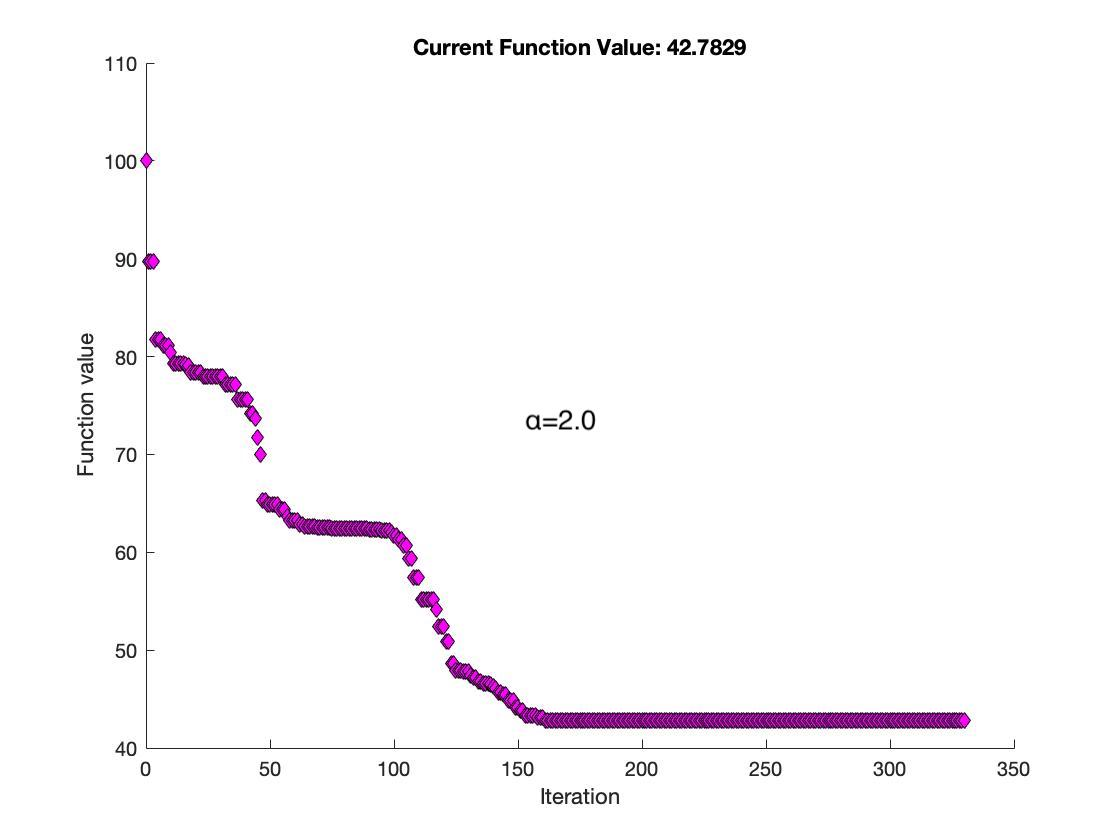
\includegraphics{CSE 848/HA1/Images/q1-Optimization Plot alpha_2.jpg} \\ 
    \end{tabular}
    }
    \caption{Reduction in function values over the iterations for $\alpha$=0.25, 1.0 and 2.0 respectively.}
    \label{fig:UncOptimizationPlot}
\end{figure}

From the results obtained using the \textit{fminsearch()} method, we can see that the algorithm works the best when $\alpha$=0.25 and it performs worse as $\alpha$ value increases. In order to investigate the validity of such results, I plotted the 2-dimensional Rastrigin function for different values of $\alpha$. These plots are presented in \autoref{fig:rastriginPlot}.\\ 

\begin{figure}[H]
    \centering
    \begin{subfigure}{0.4\textwidth}
        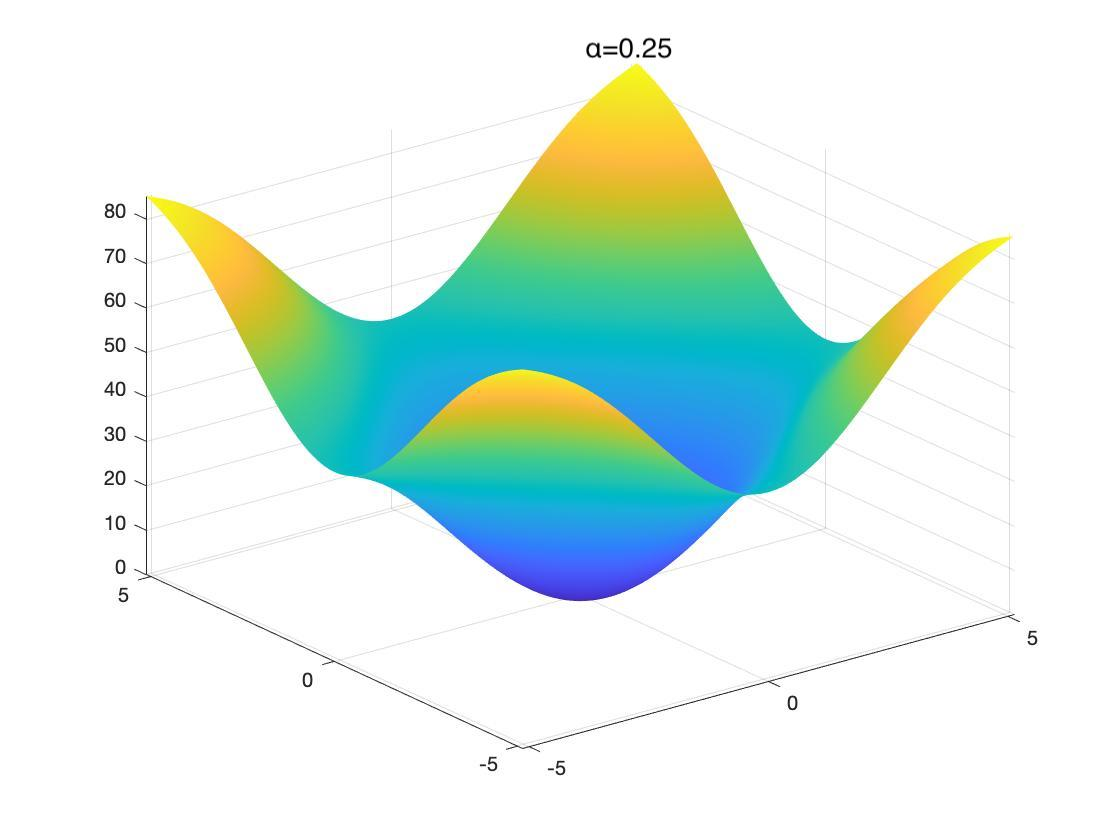
\includegraphics[width=\textwidth]{CSE 848/HA1/Images/q1-Rastrigin Plot alpha_0.25.jpg}
        \caption{}
    \end{subfigure}
    \hfill
    \begin{subfigure}{0.4\textwidth}
        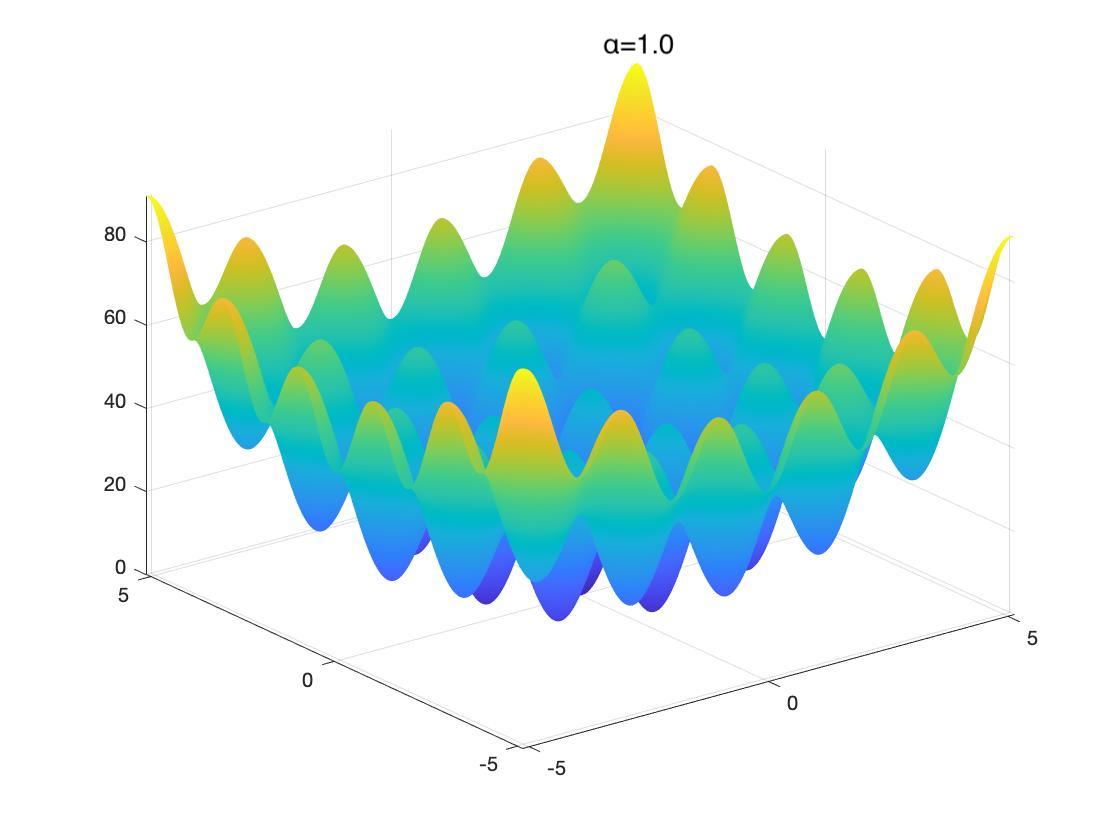
\includegraphics[width=\textwidth]{CSE 848/HA1/Images/q1-Rastrigin Plot alpha_1.0.jpg}
        \caption{}
    \end{subfigure}
    \hfill
    \begin{subfigure}{0.4\textwidth}
        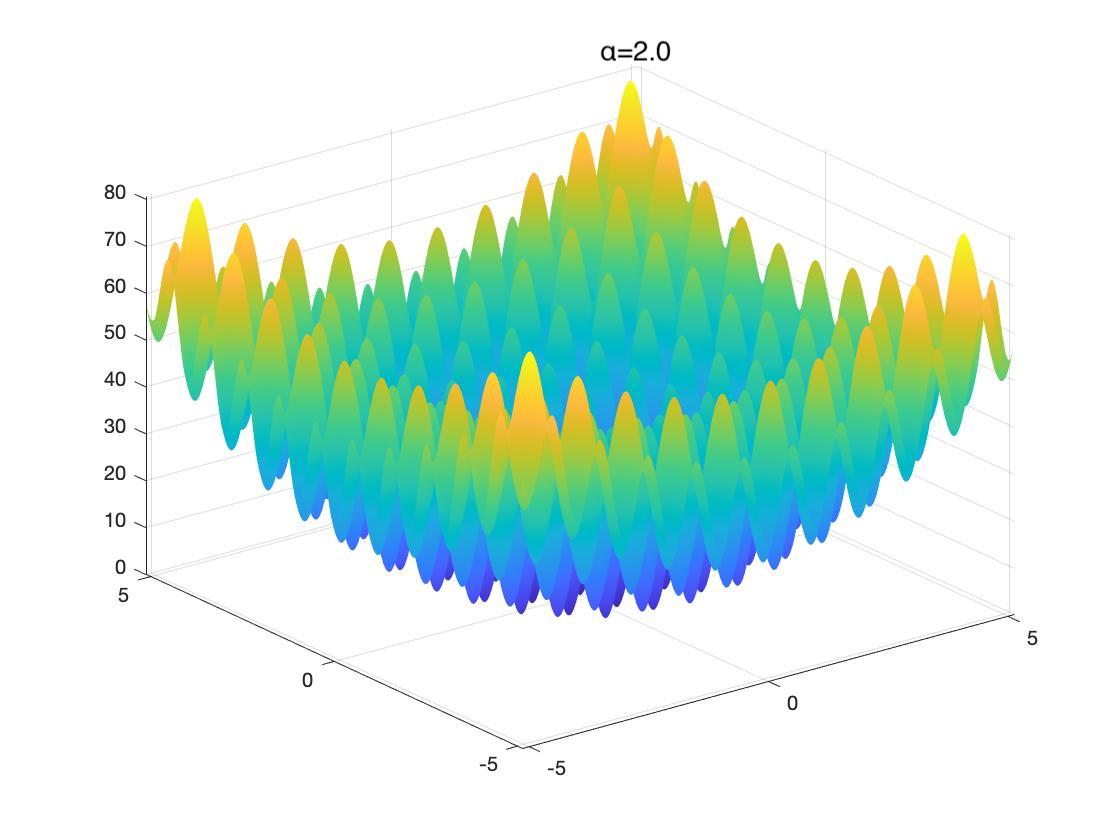
\includegraphics[width=\textwidth]{CSE 848/HA1/Images/q1-Rastrigin Plot alpha_2.0.jpg} 
        \caption{}
    \end{subfigure}
    \caption{Rastrigin function plotting for $\alpha$=0.25 (a), 1.0 (b) and 2.0 (c)  respectively.}
    \label{fig:rastriginPlot}
\end{figure}

From the plots of these functions, it is clearly visible that as the $\alpha$ value increases, the number of local optima increases as well. So, it becomes difficult for the algorithm to reach the global optimum. The final value also depends heavily on the initial point selection. If the initial point is closer to the global optimum (or its basin), the algorithm can easily find the optimum after some iterations, but if that's not the case, it can get stuck in a local optimum. This is the reason why the quality of the final solution decreases as value of $\alpha$ increases.

\newpage
2. For the following constrained minimization problem, find the minimum solution using \emph{fmincon()} routine.

\begin{align*}
        \textrm{Minimize } f(x_1,x_2) = (x_1+1)^2 +(x_2+1)^2 \\
        \textrm{Subject to: }   g_1(x_1, x_2) = (x_1-1)^2 + 4x_2^2 \leq 5,\\
                                g_2(x_1, x_2) = x_1-x_2 \geq 1,\\ 
                                g_3(x_1, x_2) = x_1 + 2x_2 \leq 2.
\end{align*}

Start with an initial solution (1, 1). Plot the history of intermediate solutions and also plot the reduction of objective values with iteration.\\

\textbf{Solution:} 
The given problem is a multivariable, constrained, non-linear minimization problem. In order to make the problem definition suitable for \textit{fmincon()} function, at first, the $\geq$ type constraint $g_2$ is modified to $\leq$ type by multiplying $-1$ to both sides of the constraint. Then the matrix formulation (for the linear part) of the problem becomes:\\

$A = \begin{bmatrix}-1 & 1\\ 1 & 2\end{bmatrix}$
, $B = \begin{bmatrix}-1\\ 2\\ \end{bmatrix}\\$

For the non-linear constraints, a function is designed to return the value of $c$ (for non-equality) and $ceq$ (for equality) whenever called. This completes the process of formulation and then \textit{fmincon()} is called using all the parameters. Starting with the point $(1,1)$, a minimum function value of $1$ is obtained at the point $x=(2e-06, -1)$. The intermediate history plot and function reduction plot are displayed in \autoref{fig:HistoryPlot(1,1)} and \autoref{fig:ConvergencePlot} respectively.

\begin{figure}[H]
    \centering
    \includegraphics[scale=0.25]{CSE 848/HA1/Images/q2-Optimization Plot(1,1).jpg}
    \caption{History of intermediate solutions for x} 
    \label{fig:HistoryPlot(1,1)}
\end{figure}

\begin{figure}[H]
    \centering
    \includegraphics[scale=0.25]{CSE 848/HA1/Images/q2-Convergence Plot.jpg}
    \caption{Reduction of f(x) over iterations} 
    \label{fig:ConvergencePlot}
\end{figure}

I tried checking the performance of the algorithm with different initial points. For this purpose, I have used two different points (2, 2) and (-1, -3). The history of the intermediate solutions for these two initial points are presented in \autoref{fig:HistoryPlot(2,2)} and \autoref{fig:HistoryPlot(-1,-3)}.

\begin{figure}[H]
    \centering
    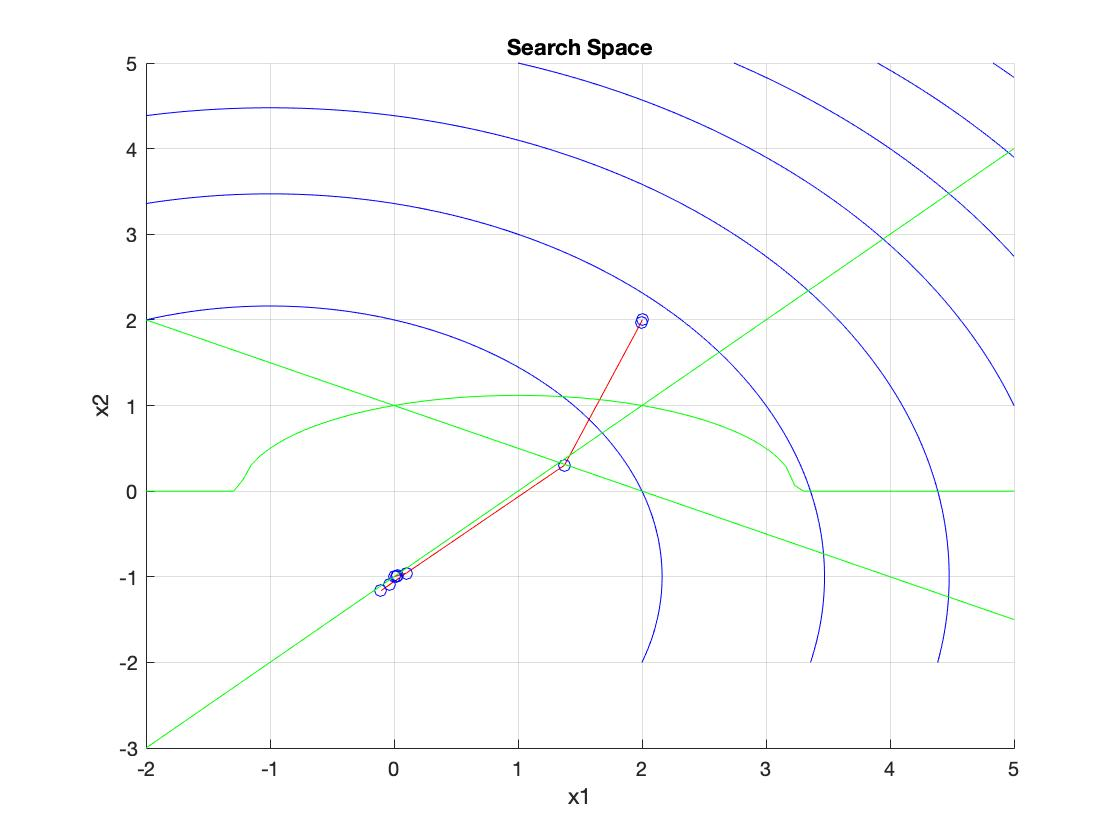
\includegraphics[scale=0.25]{CSE 848/HA1/Images/q2-Optimization Plot (2,2).jpg}
    \caption{History of intermediate solutions for x} 
    \label{fig:HistoryPlot(2,2)}
\end{figure}

\begin{figure}[H]
    \centering
    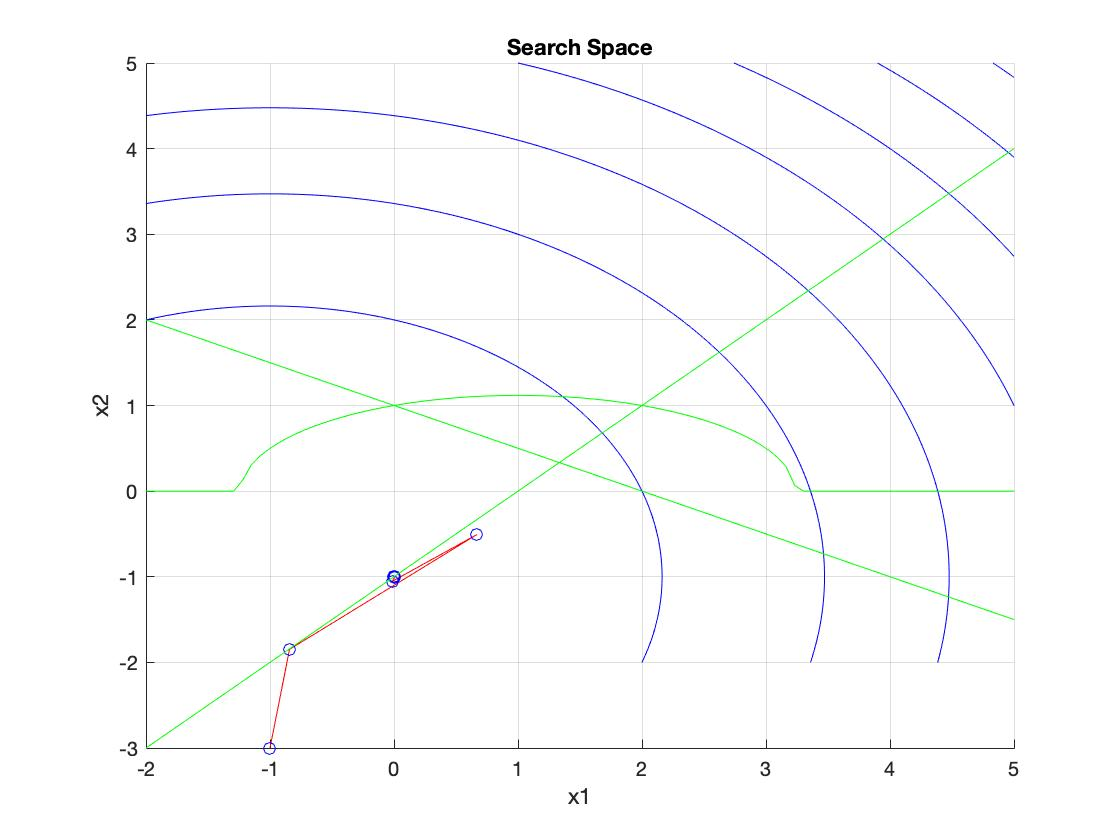
\includegraphics[scale=0.25]{CSE 848/HA1/Images/q2-Optimization Plot (-1,-3).jpg}
    \caption{History of intermediate solutions for x} 
    \label{fig:HistoryPlot(-1,-3)}
\end{figure}

The code used to obtain minimized solution for the given problem is provided below:\\

\lstinputlisting[language=Matlab]{Codes/q2.m}



\newpage
3. First, solve the following problem using \textit{linprog()} routine of Matlab.

\begin{align*}
    \textrm{Maximize } x_1 + 4x_2,\\
    \textrm{subject to: } x_1 + 5x_2 \leq 10,\\
    3x_1 + x_2 \leq 15,\\  
    x_1 + 2x_2 \geq 1,\\
    x_1,x_2 \geq 0.
\end{align*}


Then, solve it using MATLAB’s \textit{intlinprog()} routine for which the second variable is real-valued, but the first variable can only take an integer value.
Show the optimal solutions on a $x_1-x_2$ plot of feasible region and explain the validity of the obtained optimal solutions.\\

\textbf{Solution:}
The given problem is a multivariable, constrained maximization problem. In order to solve the problem using \textit{linprog()} or \textit{intlinprog()}, first certain modifications were made to the problem description to convert it to a minimization problem and make it suitable to feed to the algorithm implementations. For example, the third constraint is a $\geq$ type, so it was changed to a $\leq$ type by mutiplying both the sides by $-1$. Finally, our A, B and C matrices become:

$A = \begin{bmatrix}1 & 5\\ 3 & 1\\ -1 & -2\\\end{bmatrix}$
, $B = \begin{bmatrix}10\\ 15\\ -1\\\end{bmatrix}$
, $C = \begin{bmatrix}-1, -4\\\end{bmatrix}\\$

These matrices are fed directly to the \textit{linprog()} routine and it obtained a maximum function value of $8.9286$ with $x=(4.6429, 1.0714)$.\\

For the next part of the question, the first variable was fixed to integer values by setting $intcon=[1]$. Using \textit{intlinprog()}, a maximum function value of $8.8$ was achieved corresponding to the point $x=(4, 1.2)$. A summary of the results is provided in \autoref{tab:LinProg}.\\

\begin{table}[H]
    \centering
    \begin{tabular}{|c|c|c|}
    \hline
        \textbf{Procedure} & \textbf{Max f(x)} & \textbf{x} \\ \hline
        linprog & 8.9286 & 4.6429, 1.0714 \\ \hline
        intlinprog, intcon=[1] & 8.8 & 4, 1.2 \\ \hline
    \end{tabular}
    \caption{The max f(x) and corresponding x values obtained via \textit{linprog()} and \textit{intlinprog()}}.
    \label{tab:LinProg}
\end{table}

The results were plotted in the search space in \autoref{fig:LinProgPlot}. The green lines indicate the constraints of the problem and red lines denote the objective function. The optimal solutions of \textit{linprog()} and \textit{intlinprog()} are plotted in the graph using blue and red stars.\\

\begin{figure}[H]
    \centering
    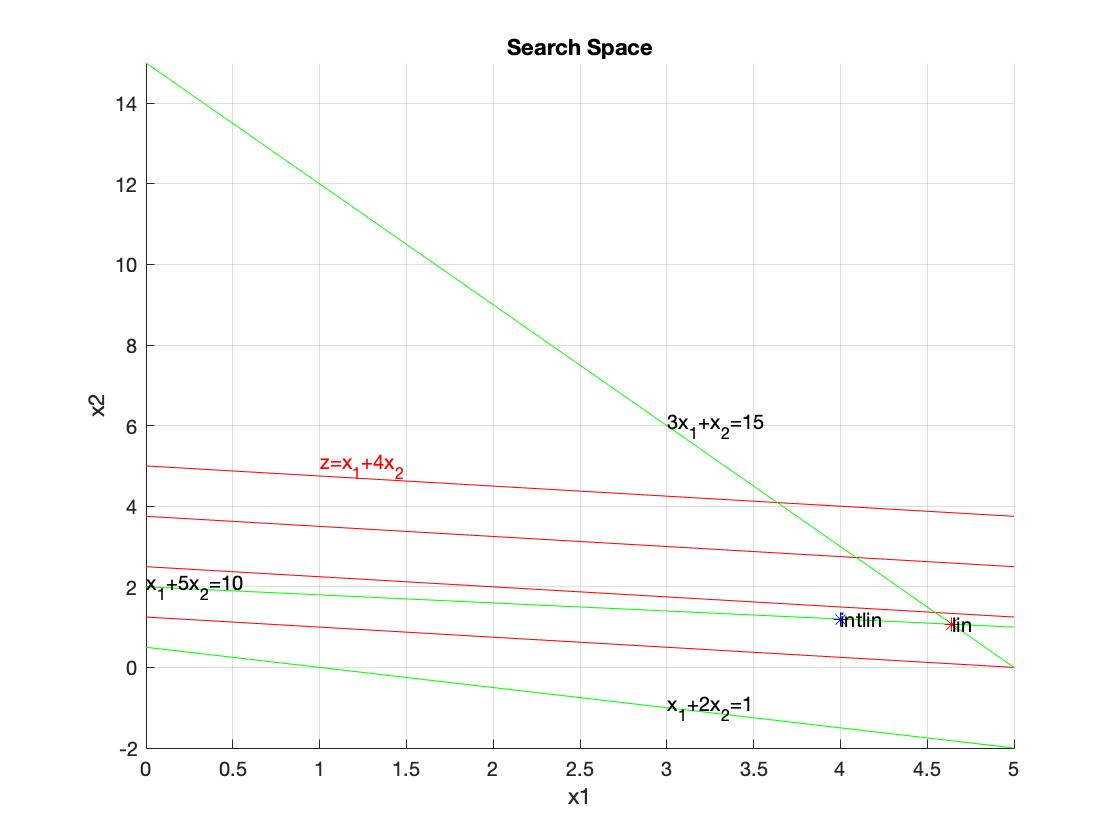
\includegraphics[scale=0.3]{CSE 848/HA1/Images/q3-LinProg Plot.jpg}
    \caption{Solution plotting in feasible region}
    \label{fig:LinProgPlot}
\end{figure}

From the obtained results, it is clear that restricting the first variable to integer values only has reduced the overall solution quality. Restricting $x_{1}$ to integer space reduces the number of values it can take. For convex optimization problems (when functions are convex and the feasible variable space is convex), the most optimal solutions are found at the corner points of the boundary. The given problem is convex in nature and the most optimal corner point does not have integral value for $x_1$ (both $x_1$ and $x_2$ are real in nature for the most optimal point) That is why restricting $x_1$ to integer values for \textit{intlinprog()} makes the optimal solution out of scope and hence we get a better solution for \textit{linprog()} over \textit{intlinprog()}.\\

The code used to solve the problem and plot the results is presented below:
\lstinputlisting[language=Matlab]{Codes/q3.m}

\end{document}

